
\subsection{Kinematisk analyse af lineær bevægelse} \label{Kinematisk analyse}
Løsningen skal sætte prikker i et arbejdsområde på \SI{200}{mm} \(\times\) \SI{150}{mm} \(\times\) \SI{50}{mm} område, hvor det ønskes, at robotten kan opnå en vilkårlig position indenfor dette område. I dette afsnit undersøges, hvordan PeJV'en skal bevæge sig, for at opfylde dette. Heraf skal PeJV'en bevæges i x-og y-retningen. Der kræves en høj præcision, i og med at en påsat prik kun må afvige med $\SI{\pm0,1}{mm}$ for at opfylde præstationskrav 1.
%Robotten skal bevæge sig i både x-og y-retningen, for at udføre sin opgave. Løsningen er den samme for de bevægelige dele i både x-og y-retningen. Drivmidlet for bevægelsen er en Nema 14 stepper motor, som sammen med en ledeskrue skaber bevægelsen. Motoren udføre et drejningsmoment på maks \(0,2\)Nm og roterer op til 2000 RPM, som sætter gang i rotationen af ledeskruen. Motoren er en stepper motor, hvilket betyder at den rotere i små steps. Én rotation er lig 360\(\degree\) og motoren har en step vinkel på 1,8\(\degree\), altså har motoren 200 steps for at opnå én rotation. Ledeskruen har en gevindstigning på \(2\)mm og en gevindhældning på \(2\)mm. 

Løsningen er den samme for de bevægelige dele i både x-og y-retningen i et kartesisk koordinatsystem. De lineære bevægelser der designes til løsningen, benævnes \textit{ Lineær x-akse} og \textit{Lineær y- og z-akse}, for bevægelsen der henholdsvis sker parallel med x-aksen og y-aksen. Disse fremgår af figur \ref{Skite af akser med pile}, hvor bevægelsesretningen er angivet med blå pile, og ledeskruernes rotation med røde pile

\begin{figure}[H]
    \centering
    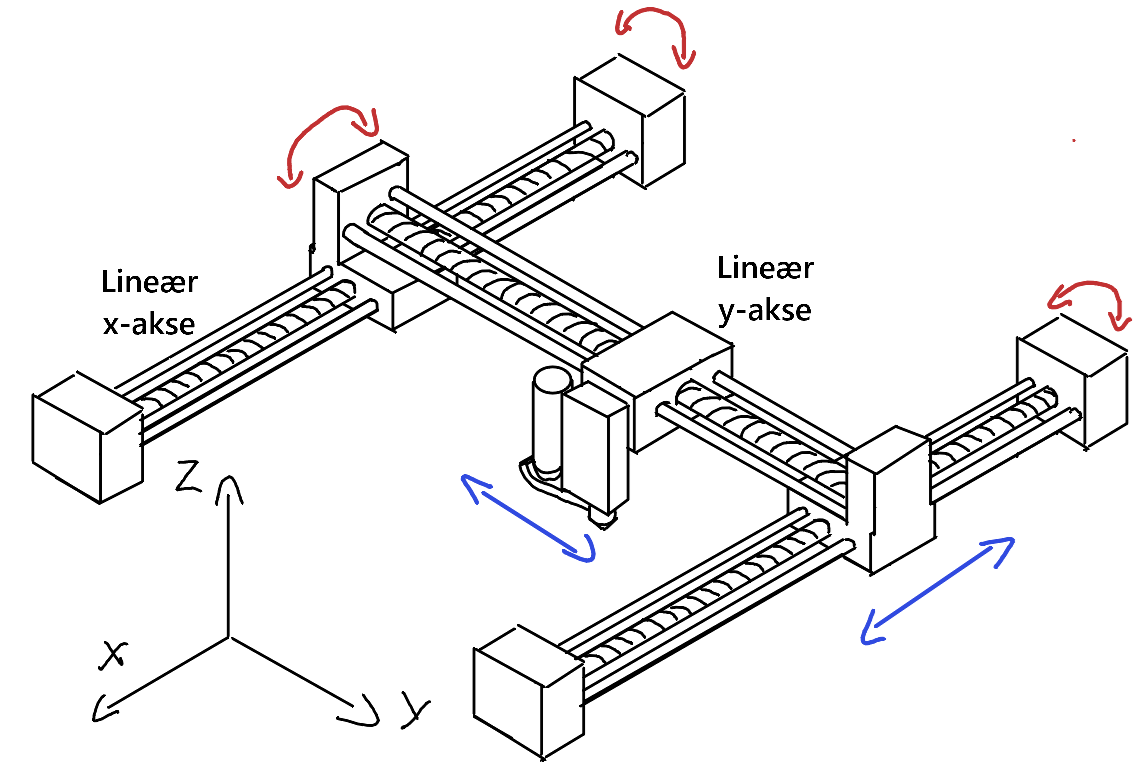
\includegraphics[width=0.8\linewidth]{Sections/6 Detaljeløsning/Media/Akser med pile.png}
    \caption{Skitse af akser, med bevægelsesretninger for de lineære akser angivet med blå pile, og ledeskruernes rotation med røde pile.}
    \label{Skite af akser med pile}
\end{figure}

Drivmidlet for bevægelsen i x-og y-aksen er en step-motor, som sammen med den udvalgte ledeskrue skaber bevægelsen. Motoren skaber et drejningsmoment, som sætter gang i rotationen af ledeskruen, der skubber to vogne langs x-aksen og PeJV'en langs y-aksen. Hvor meget akserne bevæger sig, er bestemt ud fra gevindhældningen af ledeskruen. Ledeskruen er udvalgt og i dette afsnit undersøges hvilken motor, som skal benyttes.


\begin{figure}[H]
    \centering
    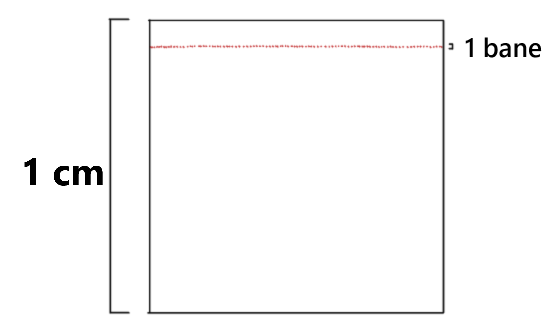
\includegraphics[width=0.4\linewidth]{Sections/6 Detaljeløsning/Media/Bane.png}
    \caption{Skite af én bane}
    \label{fig: Skite bane}
\end{figure}

I bilag \ref{Bilag - Bevægelse} gennemgås udledningen af en formel for tid pr. cm\(^2\), men også en formel for tiden det tager at køre én bane (se figur \ref{fig: Skite bane}).
En bane er defineret ud fra kvadratcentimeterens dimensioner. Da prikværktøjet kan sætte prikker under bevægelse, vil den kunne sætte en række af prikker på den tid den kan bevæge sig igennem rækken. Tiden det tager prikværktøjet at lave en række prikker fra den ene side af kvadratcentimeteren til den anden, kaldes banetiden. Banen kan ses på figur \ref{fig: Skite bane}. Prikkerne har som minimum en diameter på $\SI{0,1}{mm}$, og det er derfor muligt at placere højest 100 prikker på langs af \SI{1}{cm}, for at placere prikker på hele kvadratcentimeteren. Det er altså nødvendigt at lave 100 baner med $\SI{0,1}{mm}$ prikker af \SI{10}{mm}, for at fylde hele kvadratcentimeteren med prikker. Dette er anslået til den maksimale tid det vil tage at prikke en kvadratcentimeter, og vil bruges som overslag til tiden det vil tage at lave et speckle pattern per kvadratcentimeter.

Motoren skal igennem tre faser for at udføre sin bevægelse på én bane, henholdsvis acceleration, konstant hastighed (top hastighed) og deceleration. Dette kan skrives som:
\begin{equation}
    t_{bane}=2\cdot t_{acc}+t_{top}
\end{equation}

Hvor \(t_{bane}\) er den samlede tid det tager produktet at bevæge sig én bane. \(t_{acc}\) er tiden det tager at accelerere, men også tiden det tager og decelerere, da denne værdi er den samme, ganges denne værdi med 2. Dette udtryk udledes i \ref{Bilag - Bevægelse} til:
\begin{equation}
    t_{bane}=\dfrac{m_{l}\cdot r_{l}^2\cdot \omega}{\tau}+\dfrac{s_{bane}}{\omega\cdot O}
    \label{eq: t_bane}
\end{equation}

I ligning \ref{eq: t_bane} er \(m_{l}\) massen af ledeskruen på \SI{136}{g}, \(r_{l}\) er radius af ledeskruen på \SI{5}{mm}, \(O\) er gevindhældningen af ledeskruen på \SI{2}{mm}. Motoren har to variabler i ligningen, henholdsvis \(\tau\) og \(\omega\), hvor \(\tau\) er drejningsmomentet produceret af motoren og \(\omega\) er vinkelhastigheden. Variablen \(s_{bane}\) er længden af én bane, hvor én bane i dette tilfælde er \SI{10}{mm}, da én cm\(^2\) er \SI{10}{mm} \(\times\) \SI{10}{mm}. Dette er grundet præstationskrav nr. 8 i tabel \ref{tab:basale krav} om tid pr. cm\(^2\) og derfor skal \(t_{bane}\) som nævnt tidligere ganges med 100 for at opnå én cm\(^2\). Denne værdi  kaldes \(t_{cm^2}\)
 \begin{equation}
      t_{cm^2}=\left(\dfrac{m_{l}\cdot r_{l}^2\cdot \omega}{\tau}+\dfrac{s_{bane}}{\omega\cdot O}\right) \cdot 100
      \label{eq:tcm2}
 \end{equation}

Det vurderes at motorens vinkelhastighed skal være så høj som muligt, da en højere top hastighed har større indflydelse på tiden end acceleration. \(\omega\) er den værdi, som er interessant grundet hastigheden af den roterende ledeskrue bestemmer hvor hurtigt x-og y-aksen bevæger sig. I og med kravet på tid pr. cm\(^2\) har en værdi på maksimalt 30 sekunder, og ikke er en ukendt variabel kan \(\tau\) isoleres. 
En funktion kan derved opsættes med \(\omega\) som variabel, så der kan aflæses en minimum vinkelhastighed, som skal benyttes for at produktet kan udføre sig arbejde:
\begin{equation}
    \tau(\omega)=\dfrac{m_{l} \cdot r_{l}^2 \cdot \omega}{t_{bane} \cdot O - s_{bane}}
\end{equation}

Denne funktion plottes i et koordinatsystem med \(\omega\) ud af x-aksen og \(\tau\) op af y-asken. En minimum værdi for \(\omega\) kan nu aflæses, se figur \ref{fig: Tau-Omega plot}:
\begin{figure}[H]
    \centering
    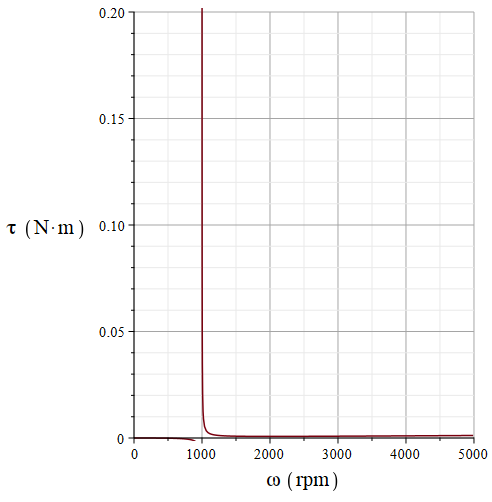
\includegraphics[width=0.5\linewidth]{Sections/6 Detaljeløsning/Media/Billeder til indspænding/tau-omegaplot.png}
    \caption{Graf over \(\tau\) som funktion af \(\omega\)}
    \label{fig: Tau-Omega plot}
\end{figure}

På figur \ref{fig: Tau-Omega plot} kan det ses at produktet vil kunne udføre sit arbejde, så længe \(\omega\) er over 1000 RPM. Kravet til valg af motor er således at den skal have en vinkelhastighed på minimum \SI{1000}{RPM} og med så højt drejningsmoment som muligt. Ud fra dette vælges en NEMA 14 step-motor. Den udvalgte motor sælges af firmaet Igus og har dimensionerne \SI{35}{mm} \(\times\) \SI{35}{mm} \(\times\) \SI{42}{mm} og kan levere et drejningsmoment op til \SI{0.18}{Nm} og en vinkelhastighed op til \SI{2000}{RPM} og vejer \SI{200}{g} \parencite{Igus2025DrylinNEMA14}. På figur \ref{fig:Udvalgte motor} kan ses et billede af den udvalgte motor. 
\begin{figure}[H]
    \centering
    \includegraphics[width=0.3\linewidth]{Sections/6 Detaljeløsning/Media/Billeder til indspænding/Nema14motor.png}
        \caption{Billede af udvalgte NEMA 14 motor. \parencite{Igus2025DrylinNEMA14}}
        \label{fig:Udvalgte motor}
\end{figure}

I bilag \ref{bilag - NEMA 14 motorkurve} ses en kurve over sammenhængen mellem drejningsmoment \(\tau\) og vinkelhastigheden \(\omega\) for den udvalgte motor. Til kommende beregninger udvælges en vinkelhastighed på \SI{2000}{RPM}, hvor drejningsmomentet kan aflæses til \SI{0.12}{Nm}. 

Disse nye værdier for \(\tau\) og \(\omega\) kan nu indsættes i den oprindelige formel \ref{eq:tcm2}, for at finde tiden det tager produktet og udføre sin opgave på én cm\(^2\)
\begin{equation}
    t_{cm^2}=\left(\dfrac{m_{l}\cdot r_{l}^2\cdot \omega}{\tau}+\dfrac{s_{bane}}{\omega\cdot O}\right) \cdot 100
\end{equation}

\(t_{cm^2}\) udregnes med de nye værdier til at være \SI{15,1}{s}, hvilket betyder at præstationskrav nr. 8 opfyldes, da \(t_{cm^2}\) befinder sig under grænseværdien på 30 sekunder.

Nu hvor en motor er blevet udvalgt kan en acceleration bestemmes, samt en tophastighed. I bilag \ref{Bilag - Bevægelse} er accelerationen givet af to formler: \\
\begin{equation}
\begin{aligned}
a = \alpha \cdot O \hspace{20mm} \text{hvor} \hspace{20mm} \alpha = \dfrac{\tau}{m_{l}\cdot r_{l}^2}
\end{aligned}
\end{equation}

Udtrykket for \(\alpha\) indsættes i formlen for accelerationen:
\begin{equation}
    a=\dfrac{\tau}{m_{l}\cdot r_{l}^2}\cdot O
\end{equation}

Med en gevindhældning \(O\) på \SI{2}{mm} og en radius \(r_{l}\) af ledeskruen på \SI{5}{mm} fås en acceleration på \SI{70,8}{m/s^2}. Tophastigheden udregnes ved: \(v=\omega\cdot O\) og er \SI{6,67}{cm/s} eller \SI{0,07}{m/s}

Motoren har også en relevans for præcisionen af produktet. NEMA 14 motoren er en step-motor, hvilket betyder, at motoren kører i små steps. Den udvalgte motor har ifølge \parencite{Igus2025DrylinNEMA14} en step vinkel på 1,8\(\degree\) og da én rotation er 360\(\degree\) har motoren 200 steps til at udføre én rotation, denne værdi kaldes \(n_{step}\). Præcisionen kan derved bestemmes ud fra \(n_{step}\) og gevindhældningen \(O\)
\begin{equation}
    \delta=\dfrac{O}{n_{step}}
\end{equation}

Dette giver en præcision ned til \SI{0,01}{mm}. Motoren opflyder præstationskrav 3. Det undersøges senere om denne værdi også er overholdt i forhold til udbøjning.


\begin{comment}
    \renewcommand{\arraystretch}{1.3}
\begin{table}[H]
\setlength{\tabcolsep}{20pt}
 \centering
  \caption{Variabelliste}
 \begin{tabular}{|c c|} \hline
   
 \rowcolor{aaublue} \multicolumn{1}{|c}{\textcolor{white}{\textbf{Variabel}}} &  \multicolumn{1}{c|}{\textcolor{white}{\textbf{Værdi}}}  \\\hline
 \(t_{cm^2}\) & \SI{15,1}{s}\\\hline
 \(\tau\) & \SI{0,12}{Nm}\\\hline
 \(\omega\) & \SI{2000}{RPM}\\\hline
 \(a\) & \SI{70,8}{m/s^2}\\\hline
 \(\delta\) & \SI{0,01}{mm}\\\hline
 \end{tabular}
 \label{tab: variabelliste}
\end{table}
\end{comment}
\begin{comment}
Ledeskruen sidder inde i motoren, og rotation igangsættes af drejemomentet leveret af motoren og skruen omdanner den roterende kraft til lineær bevægelse. Ledeskruen antages at have en effektivitet på omkring 50\% grundet friktionen på gevindet, hvilket betyder at 50\% af den roterende kraft bliver omdannet til lineær bevægelse.
\begin{figure}[H]
    \centering
    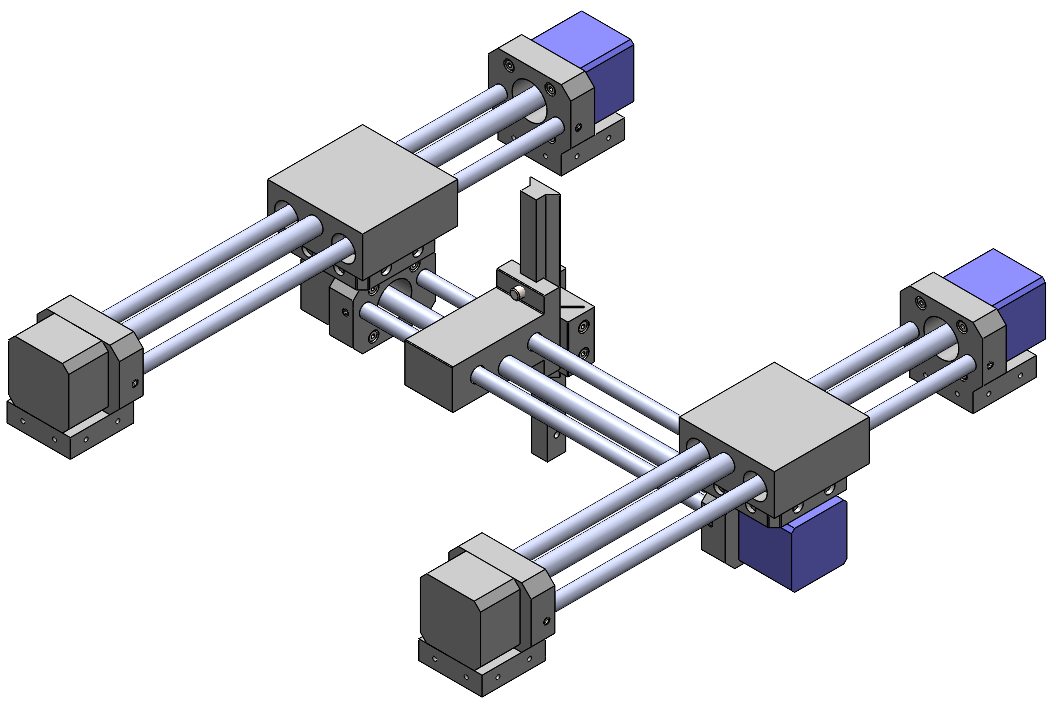
\includegraphics[width=0.8\linewidth]{Sections/6 Detaljeløsning/Media/x,y,z akse.png}
    \caption{Oversigt over x-og y-aksen}
    \label{fig: overview x-y-akse}
\end{figure} 

På billedet kan det ses, at en vogn skal køre frem og tilbage på de to akser. Dette gøres ved at have et gevind inde i vognen, hvor rotationen af ledeskruen vil bevæge vognen frem og tilbage ved \(2\)mm pr. rotation. Der er to følgestænger, som stabiliserer vognen, samt vognen har påsat fire lineære lejre, som mindsker friktion mellem vogn og følgestænger.

Denne konstruktion på henholdsvis x-og y-aksen skal kunne bevæge sig \(200\)mm \(\times\) \(150\)mm, som arbejdsområdet kræver, men har også et krav på tid pr. cm\(^2\), som lyder på 30 sekunder, som begge kan findes i tabel \ref{tab:basale krav}.  Først skal det udregnes, hvor hurtigt robotten kan bevæge sig. Dette kan gøres ved følgende formel:
\begin{equation}
    v=\omega \cdot O
\end{equation}

I formlen for hastigheden er \(\omega\) lig antallet af omdrejninger, som motoren producerer pr. minut, altså 2000 og \(O\) er gevindhældningen på ledeskruen på \(2\)mm. Hastigheden, som ledeskruen kan bevæge sig, er lig \(0,05 \dfrac{m}{s}\).

Dernæst skal tiden fastlægges, både for én bane og dernæst pr. cm\(^2\), hvor én bane er den ene siden af én cm\(^2\), altså \(10\)mm. Der startes med at identificere de faser, som robotten skal igennem, under en bevægelse. Når robotten bevæger sig, skal den igennem tre faser, henholdsvis: Acceleration, bevægelse ved konstant hastighed (top hastighed) og deceleration. Det vil sige, at når tiden skal findes for én bane, kan \(t_{bane}\) defineres som tiden det tager og accelerere og decelerere, samt tiden i top hastighed. Det kan skrives som:
\begin{equation}
\label{Formel:t_{bane}}
    t_{bane}=2 \cdot t_{acc}+t_{top}
\end{equation}

\(t_{bane}\) er defineret udfra, tiden robotten bruger på at accelerere, \(t_{acc}\), samt tiden robotten er i top hastighed, \(t_{top}\). Definitionen af disse to kan findes i bilag \ref{Bilag - Bevægelse} og indsættes på deres respektive pladser i formel \ref{Formel:t_{bane}}:
\begin{equation}
    t_{bane}=2\cdot(\dfrac{m\cdot r^2\cdot \omega}{\tau})+(\dfrac{s_{bane}}{\omega\cdot O}-\dfrac{m\cdot r^2\cdot \omega}{\tau})
\end{equation}
Dette forkortes:
\begin{equation}
    t_{bane}=\dfrac{m\cdot r^2\cdot \omega}{\tau}+\dfrac{s_{bane}}{\omega\cdot O}
\end{equation}

Her er \(m\) lig massen af ledeskruen på \(136\)g. \(r\) er lig radiussen af ledeskruen på \(5\)mm og \(s_{bane}\) er længden af én bane på \(10\)mm. 
Da en cm\(^2\) er defineret som \(10\)mm \(\times\) \(10\)mm, betyder det, at længden af én bane, er lig 10mm. Tykkelsen af en bane er lig \(0,1\)mm, da det er den mindste priktykkelse, som robotten skal kunne placere. Det vil betyde, at \(t_{bane}\) skal ganges med 100, da der skal 100 baner til for at opnå \(1\)cm\(^2\):
\begin{equation}
    t_{cm^2}=t_{bane}\times 100
\end{equation}

Tiden pr. cm\(^2\) er lig \(15,1\)s, hvilket betyder, at kravet om tidsforbrug pr. cm\(^2\) på 30 sekunder er opfyldt og at robotten bevæger sig, som den skal i x-og y-retningen. Den fulde formeludledning med symboler kan findes i bilag \ref{Bilag - Bevægelse}.
\end{comment}
